\begin{abstract} This extended abstract studies whether the MuJoCo Playground
zero-shot sim-to-real recipe for humanoid joystick locomotion extends to the
ROBOTIS OP3 platform. MuJoCo Playground treats OP3 as a first-class humanoid
robot alongside Berkeley Humanoid, Unitree H1/G1, and Booster T1; however,
unlike these larger robotic platforms, zero-shot transfer to the OP3 hardware
was not reported in \citet{Zakka2025-demonstrating-mujoco-playground}. Our
contribution is an engineering audit of the path from the OP3 policy distributed
by MuJoCo Playground in simulation to an OP3-facing deployment stack, with
sim-to-sim testing through the ROBOTIS OP3 ROS~2 framework as a preliminary step
toward eventual sim-to-real deployment. We present the work as the first step of
a longer research programme that aims to combine reinforcement-learning
policies, motion scripts, and analytical control to improve the OP3's
football-playing skills. The central finding is that small mismatches in
observation conventions, command filtering, actuator stiffness, and
contact-friction modelling can determine whether a policy that walks in
simulation remains meaningful when moved through the deployment stack and onto
hardware.  \end{abstract}

\vspace{0.4em}
\noindent\textbf{Keywords:} ROBOTIS OP3; MuJoCo Playground; Webots; ROS~2; humanoid locomotion; sim-to-sim; sim-to-real.

\section{Motivation}

MuJoCo Playground \citep{Zakka2025-demonstrating-mujoco-playground} reduces the
friction between simulator construction, policy training, and real-robot
deployment. The authors present it as a fully open-source framework, built on
MJX (MuJoCo's JAX-accelerated branch), that lets users install a standard
robot-learning stack, train policies in minutes of training on a single GPU, and
iterate between simulated environments and hardware. According to the authors,
its design offers GPU-accelerated physics, on-device batch rendering, and
ready-made locomotion and manipulation environments, so that subsequent research
effort can focus on robot behaviour and sim-to-real fidelity rather than
rebuilding the simulation infrastructure for one platform at a time.

Reinforcement learning has been used to train humanoid locomotion policies that
transfer to hardware in this style
\citep{Rudin2022-learning-to-walk-in-minutes-massively-parallel-deep-reinforcement-learning,Gu2024-humanoid-gym-reinforcement-learning-humanoid-robot-zero-shot-sim-to-real-transfer,Zakka2025-demonstrating-mujoco-playground},
but successful transfer depends on whether the training simulator, the exported
policy, the middleware, and the robot control stack reproduce the physical
robot's closed-loop dynamics with enough fidelity that the trained policy still
walks. Playground is a useful test case here because it is both a canonical
reproduction target and a strong sim-to-real claim: the authors describe
zero-shot transfer across six robot platforms in under eight weeks, with
deployment through ONNX Runtime (the Open Neural Network Exchange runtime, a
portable inference format) at 50~Hz, ROS~2 control, real-time C++ control, and a
model-based body-state estimator
\citep{Zakka2025-demonstrating-mujoco-playground}.

Related frameworks are converging on similar abstractions for humanoid
locomotion training and deployment, which makes the question of how reliably
those abstractions reproduce on a given physical platform a timely one. Isaac
Lab
\citep{Mittal2025-isaac-lab-gpu-accelerated-simulation-framework-multi-modal-robot-learning}
and ROBOTIS Lab
\citep{ROBOTIS2026-robotis-lab-reinforcement-learning-imitation-learning-robotis-robots}
provide Isaac-Sim-based robot-learning stacks for legged and humanoid robots;
Humanoid-Gym
\citep{Gu2024-humanoid-gym-reinforcement-learning-humanoid-robot-zero-shot-sim-to-real-transfer}
and \texttt{legged-gym}
\citep{Rudin2022-learning-to-walk-in-minutes-massively-parallel-deep-reinforcement-learning}
situate GPU-parallel locomotion training and sim-to-real transfer in the
legged-robot literature.

The ROBOTIS OP3 is one of the humanoid robots distributed in the Playground task
family, but its hardware was not included in the zero-shot transfer demonstration. This
makes OP3 an interesting case for SPECS: if the shared joystick abstraction
transfers to the physical OP3 we will be able to combine
reinforcement-learning policies, motion scripts, and analytical control to
improve the OP3's football-playing skills.  We use this first study to map
the fidelity gaps that any next step will need to close.

\section{Pipeline}

The OP3 is defined in MuJoCo using an MJCF (MuJoCo's XML scene-description
format) model from MuJoCo Menagerie's curated collection, following the
Playground \texttt{Op3Joystick} task
\citep{Zakka2022-mujoco-menagerie-collection-high-quality-simulation-models,Zakka2025-demonstrating-mujoco-playground,GoogleDeepMind2025-mujoco-playground-gpu-accelerated-robot-learning-sim-to-real-transfer}.
The model is simulated in MJX (MuJoCo's JAX-accelerated physics branch) on GPU
and a policy is trained with Proximal Policy Optimisation (PPO) implemented in
Brax. The policy is queried at $50$~Hz on a 147-dimensional observation (three
stacked frames of joint state, IMU readings, command velocity, and previous
action); actions are 20-dimensional joint-position offsets relative to the
\texttt{stand\_bent\_knees} default pose, one per actuated degree of freedom of
the OP3. The training rewards for linear velocity and yaw from the standard MuJoCo Playground locomotion
family are
\begin{equation}
\label{eq:reward-tracking}
r_{\text{lin}} = w_{\text{lin}} \exp\!\big(-\lVert c_{xy} - v^{\text{body}}_{xy} \rVert^2 / \sigma\big), \qquad
r_{\text{yaw}} = w_{\text{yaw}} \exp\!\big(-(c_\omega - \omega_z)^2 / \sigma\big),
\end{equation}
with $w_{\text{lin}} = 1.5$, $w_{\text{yaw}} = 0.8$, and tracking width
$\sigma = 0.25$. The trained policy is exported to ONNX (Open Neural Network Exchange) and served by a ROS~2 node that drives the OP3 in Webots through the ROBOTIS OP3 ROS~2 framework as a sim-to-sim diagnostic before any hardware run.

\begin{figure}[t]
  \begin{minipage}[b]{0.42\textwidth}
    \begin{subfigure}[b]{0.46\linewidth}
      \centering
      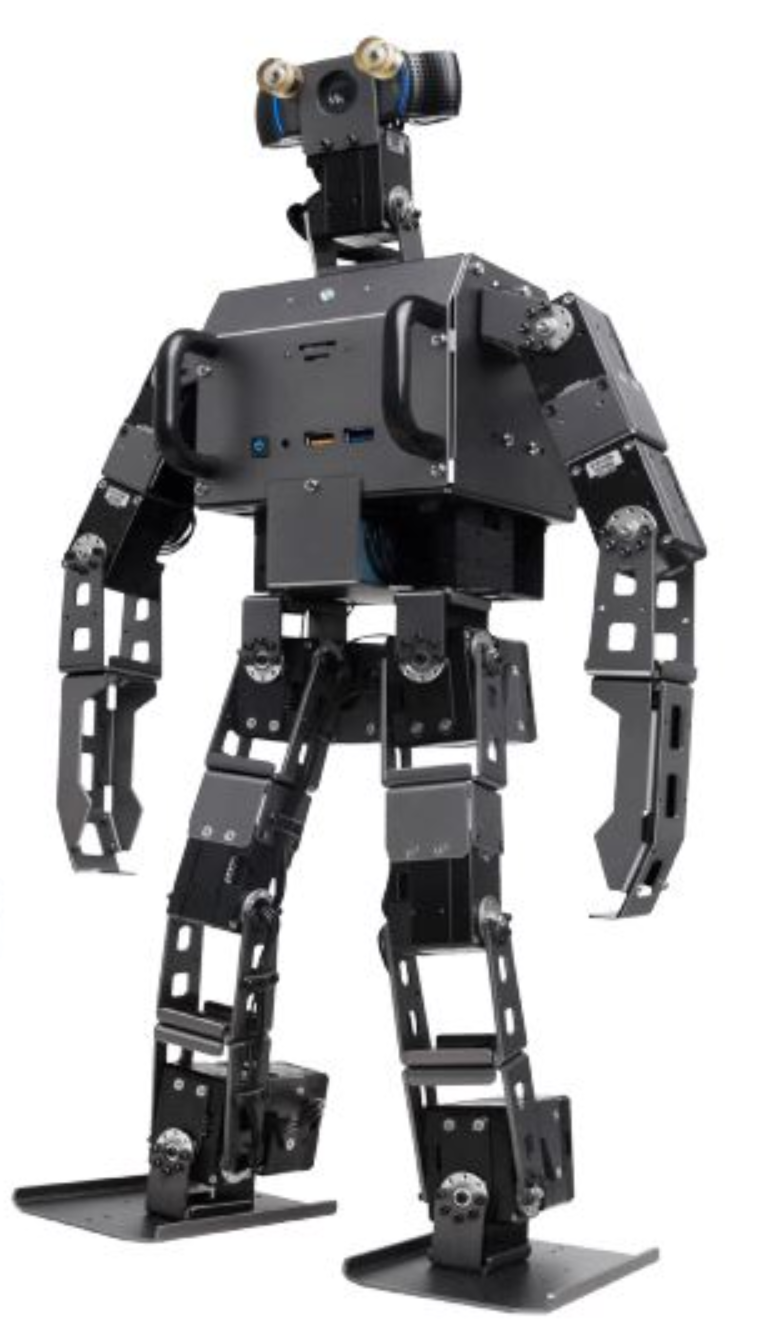
\includegraphics[width=\linewidth,keepaspectratio]{figures/OP3-real.png}
      \caption{Physical OP3.}
      \label{fig:pipeline-real}
    \end{subfigure}\hspace{0.04\linewidth}%
    \begin{subfigure}[b]{0.46\linewidth}
      \centering
      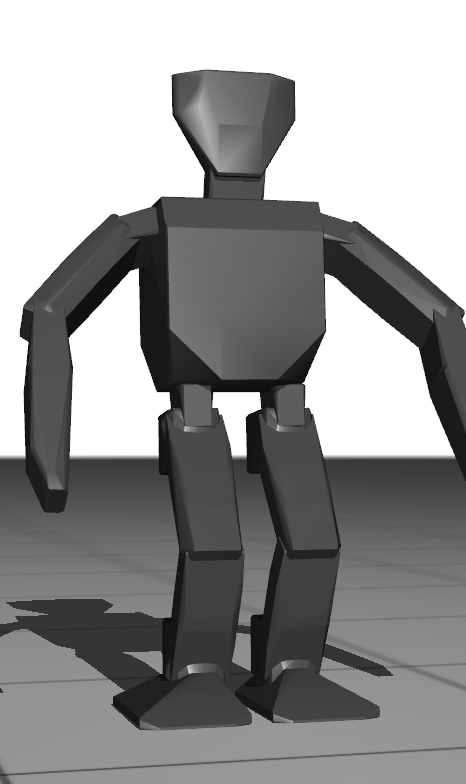
\includegraphics[width=\linewidth,keepaspectratio]{figures/op3-mujoco.png}
      \caption{OP3 in MuJoCo.}
      \label{fig:pipeline-mujoco}
    \end{subfigure}
    \captionof{figure}{The MuJoCo Playground model (b) is simplified for fast RL training. Mass distribution, contact geometry, and visual detail differ substantially from the physical robot (a), though actuator and joint conventions are nominally aligned.}
    \label{fig:pipeline}
  \end{minipage}\hfill
  \begin{minipage}[b]{0.54\textwidth}
    \centering
    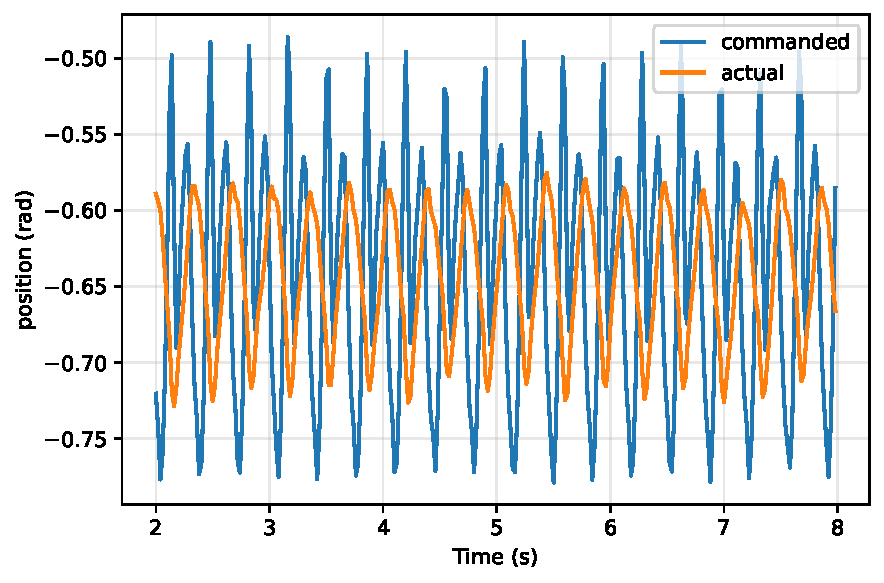
\includegraphics[width=\linewidth,keepaspectratio]{figures/joint_tracking_mujoco_ankle.pdf}
    \captionof{figure}{Right ankle-pitch tracking under a $+0.5$~m/s forward command in MuJoCo, seed-42 stage-2b ONNX. The actual joint (orange) follows the commanded target (blue) with a small consistent phase offset of order $60$~ms. The first two seconds of the rollout are excluded so the gait has reached steady state.}
    \label{fig:sim2sim}
  \end{minipage}
\end{figure}

\section{Through sim-to-sim towards sim-to-real} 

Before deploying on hardware, we introduce a sim-to-sim validation stage in
which the trained policy is executed in both MuJoCo (training environment) and
Webots (deployment simulator). The purpose is not to claim that Webots is more
accurate than MuJoCo, but to test whether the exported ONNX policy and ROS~2
policy node can drive an OP3 model outside the original training simulator. The
policy is first verified in MuJoCo to reproduce the reference joystick
locomotion behaviour. The same exported ONNX is then deployed in Webots through
the ROS~2 policy node. This setup isolates differences arising from simulator
dynamics. In particular, differences observed between MuJoCo and Webots can be
attributed to actuator modelling (e.g., stiffness and damping), contact
dynamics, and timestep integration, rather than joint ordering or coordinate
conventions. We compare the two simulators under identical joystick commands
using joint position tracking (target versus actual), tracking error over time,
torque over time, and step response.

A useful diagnostic emerges already from MuJoCo. \autoref{fig:sim2sim} replays
the trained policy at $+0.5$~m/s forward command in the training simulator: the
actual joint position lags the commanded target by a small consistent offset (of
order $60$~ms) and follows with a slightly reduced amplitude. This is not
tracking error — motors take a moment to move, joints have inertia, and the
physics has its own natural delay and damping. The PPO reward terms
(\autoref{eq:reward-tracking}) reward body-velocity tracking, not joint
tracking, so the policy is free to issue joint targets that, given this offset,
produce the desired body motion. The offset is therefore a signature of the
actuator-and-physics block that the policy was trained on, and walking succeeds
with the policy working through this lag rather than against it. A different
simulator (Webots) or the physical robot has its own lag and damping, and the
same policy commands then produce a different actual trajectory and a different
body trajectory.


The same diagnostic exposes a concrete sim-to-real fidelity question. The
Playground default OP3 stiffness, $k_p = 21.1$, is too soft for the measured
physical robot: in a static walk-ready hold the real OP3 keeps every joint
within roughly $0.1$--$0.2°$ over five seconds, while the simulator at this gain
yields visibly under gravity. Raising $k_p$ to about $100$ closes most of the
static gap but does not fully recover the real robot's stiffness. Doing so also
changes the closed-loop bandwidth shown in \autoref{fig:sim2sim}, so any
stiffness adjustment at the actuator block must be paired with a re-export or,
more honestly, a retraining cycle at the new gain — otherwise the policy is
asked to drive a closed-loop it was not trained against.

Hardware deployment of the trained policy was attempted but did not yet produce stable walking. The proximate cause is a timing mismatch in the control stack: the policy is queried every $20$~ms and assumes the actuator response visible in \autoref{fig:sim2sim}, while the ROBOTIS framework interposes a millisecond-scale Dynamixel control cycle, a configurable trajectory generator in the \texttt{direct\_control\_module}, and per-module differences in how commanded joint targets are dispatched. The constraint is not the time any single joint takes to reach its commanded angle in isolation, but that all twenty joints arrive at their commanded angles together, in phase with the policy's gait timing — a property the policy was trained against in MuJoCo and that the deployment chain does not yet preserve. The natural next step is domain randomisation over actuator gains, action delay, and trajectory-smoothing parameters, so the policy no longer depends on a single closed-loop signature; the phase offset baked into today's policy (\autoref{fig:sim2sim}) is precisely the property that randomised training would broaden.

\section{Yaw motion fine tuning}

Football play places high demands on yaw control: the robot must reorient
quickly to face the ball, line up a kick, and track moving teammates and
opponents, so a wider yaw command range than the published default is well
motivated. Following Appendix~C of
\citet{Zakka2025-demonstrating-mujoco-playground} we ran three independent runs
through three stages: \textit{stage 1} ($100$\,M steps at the published default)
intended to learn baseline locomotion; \textit{stage 2a} ($50$\,M steps)
widening the yaw command range from $\pm 0.7$ to $\pm 2\pi$~rad/s — the only
change, with reward weights and other hyperparameter held constant — to
push the policy onto wider turns; and \textit{stage 2b} ($50$\,M steps)
continuing the same fine-tune to test whether what stage 2a disturbed could be
recovered. Whether re-tuning the published hyperparameters is needed for the OP3
specifically is left for follow-up.

Within stage 1, the policy first acquires linear-velocity tracking — forward, backward, and strafing — consistent with the $w_{\text{lin}}/w_{\text{yaw}} = 1.875$ ratio in \autoref{eq:reward-tracking}, which rewards translation almost twice as strongly as rotation. \autoref{fig:results} shows total episode reward (left panel) and the yaw-tracking reward component (right panel) across all three stages. Both panels show the same shape: a dip at the stage-1 to stage-2a boundary, partial recovery across stage 2b. We read this as the policy re-balancing after the wider yaw sampling — more episodes now demand turning on the spot, where the linear-velocity term contributes less reward and the yaw-tracking term is itself depressed until the policy adapts to the expanded command range, so both metrics drop together. The shaded band on the left is wider because total reward sums many terms whose seed-to-seed variance accumulates, while the yaw term is a single, more tightly constrained component.

What stage 2 buys, and what it costs: averaged across the three runs, fast-yaw tracking error ($\pm 1.5$~rad/s) falls by $1$--$7$~pp while slow-yaw error ($\pm 0.5$~rad/s) inflates by $4$--$73$~pp; one stage-2a run reached $95\%$ slow-yaw error with the body leaning side-to-side rather than turning under a $0.5$~rad/s command. Stage 2b partially recovers slow-yaw quality on every run, but no run returns to stage-1 levels. With three runs we treat these as observed tendencies. A second feature of \autoref{eq:reward-tracking} explains the lean failure: $r_{\text{yaw}}$ is a per-step rate gap, satisfied by a body that oscillates symmetrically around the commanded yaw rate as well as by one that turns. The lesson for the longer programme is that range expansion alone is not free; the curriculum buys speed at the edge by giving up precision at the centre, and the reward shape admits at least one local optimum in which the body satisfies the metric without doing what we wanted.

\begin{figure}[t]
  \centering
  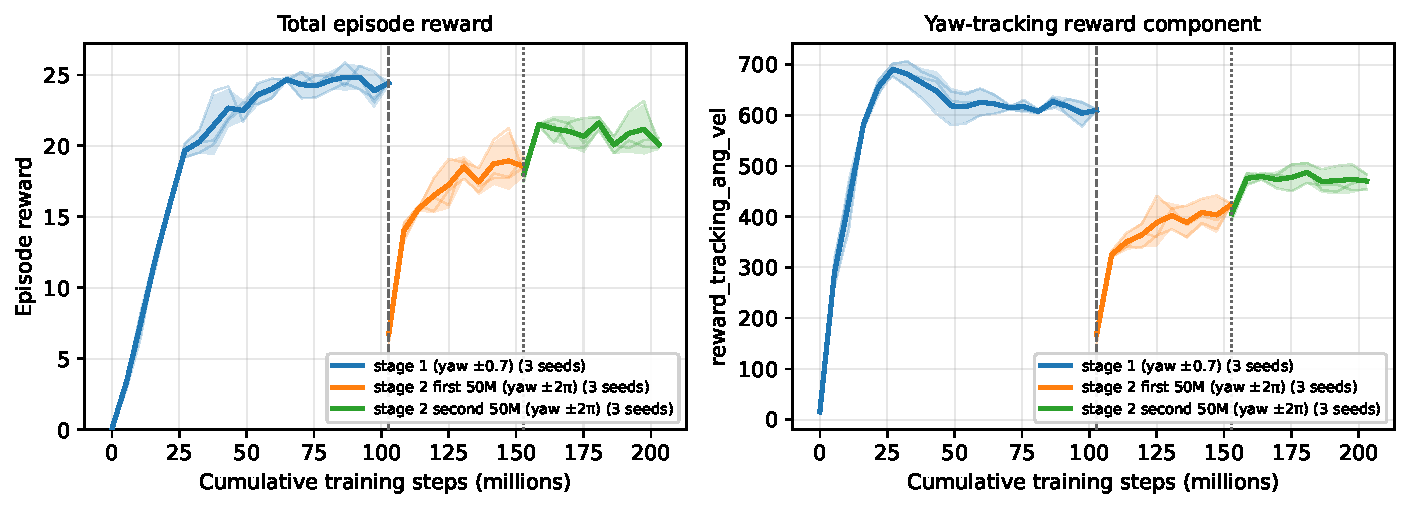
\includegraphics[width=\textwidth,keepaspectratio]{figures/three_stage_curriculum.pdf}
  \caption{Reward curves across the $200$\,M cumulative-step replication of the joystick fine-tune curriculum from \citet{Zakka2025-demonstrating-mujoco-playground} Appendix~C, three independent runs per stage; mean and one-standard-deviation band, with thin per-run lines underneath. Vertical dashed line: stage-1 to stage-2a boundary, where the yaw command range is expanded from $\pm 0.7$ to $\pm 2\pi$~rad/s. Vertical dotted line: stage-2a to stage-2b, where the same fine-tune is continued. Left panel: total episode reward. Right panel: angular-velocity tracking reward component.}
  \label{fig:results}
\end{figure}

\section{Contribution and future work}

We trace a candidate path from the public MuJoCo Playground OP3 task through a
sim-to-sim diagnostic in Webots, and identify three concrete obstacles that any
sim-to-real attempt on the OP3 will need to close: actuator stiffness,
closed-loop bandwidth, and control-stack timing. Our goal is sim-to-real walking
on the physical OP3. The immediate next step is a training cycle with domain
randomisation over actuator gains, action delay, and trajectory-smoothing
parameters, so the deployed policy no longer depends on the single closed-loop
signature of the training simulator. Beyond walking, the longer programme
replaces the OP3's mode-switched walking, action-playback, and get-up modules
with a single reinforcement-learned policy with fall recovery such that it adapts to 
disturbances within the same gait.

